\documentclass[11pt,a4paper]{article}

\usepackage{iftex}
\ifPDFTeX
  \usepackage[utf8]{inputenc}
  \usepackage[T1]{fontenc}
  \usepackage{lmodern}
\else
  \usepackage{fontspec}
  \setmainfont{Liberation Serif}
\fi
\usepackage[czech]{babel}
\usepackage[margin=25mm]{geometry}
\usepackage{pdfpages}
\usepackage{graphicx}
\usepackage[hidelinks]{hyperref}

\title{\textbf{Omnia}\\[4pt]
\large jeden svazek, žádná nová věta}
\author{Jan Mikulík}
\date{19. listopadu 2026}

\begin{document}
\maketitle

\noindent
Tři dodané soubory jsou tu jedenkrát.
\emph{Principia academica L'amour} a \emph{Golden Sphere} jsou už součástí souhrnného vydání
\emph{Principia GoldenSphere}.
Tisknout je znovu před sborníkem by znamenalo říct totéž třikrát.
Sborník proto následuje celý: dopis, sféra, Eulerův horizont a paměť návratu.

Podmíněný rámec se nemění.
Stejné jméno není stejná věc.
Stejný modul není stejná fáze.
Stejný součet není stejné místo účtu.
Krok je právě tehdy, když je dodán svědek.
Hypotéza 9, láska jako operátor, vědomí a poloha nul \(\xi\) nejsou věty tohoto svazku.
Ostatní je text, který sborník už obsahuje.

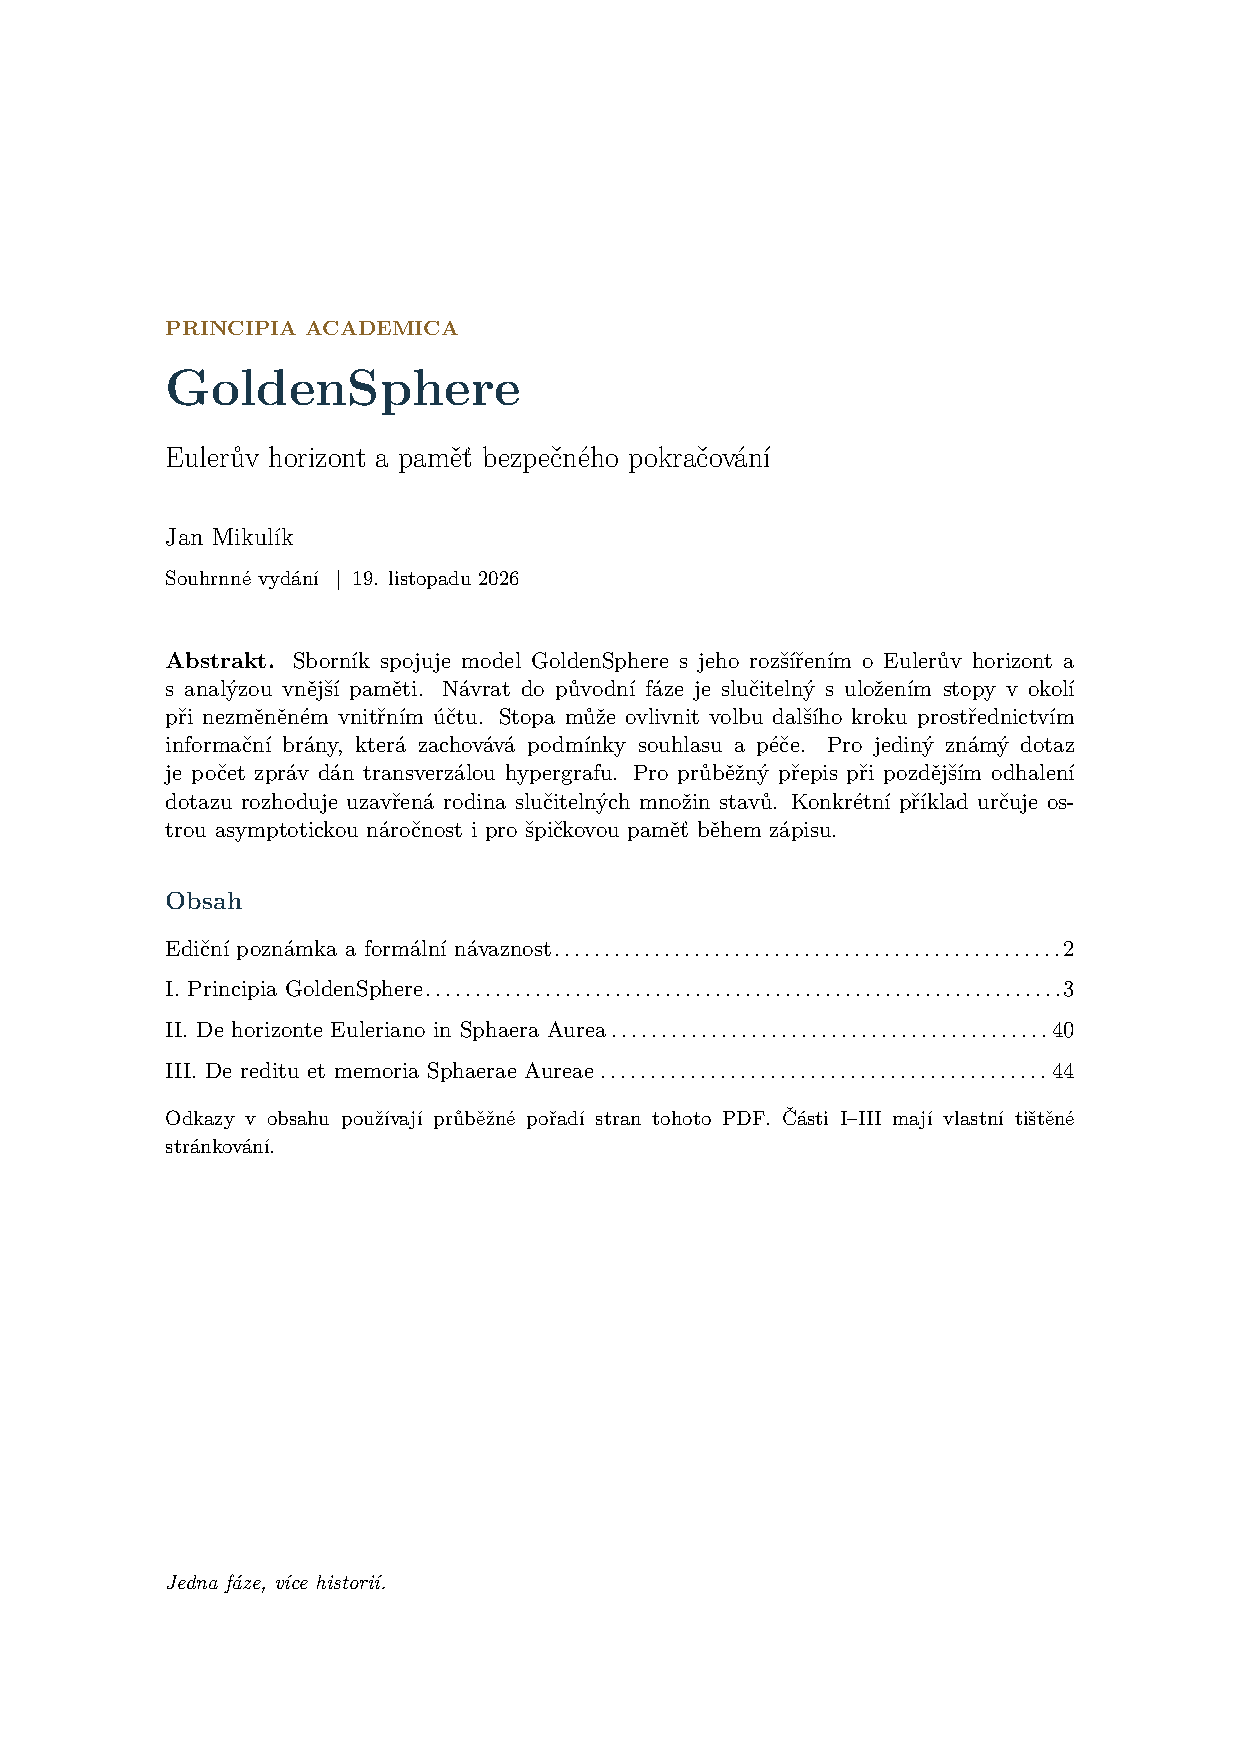
\includepdf[pages=-]{Principia_GoldenSphere_Collecta.pdf}

\clearpage
\thispagestyle{empty}
\begin{center}

\includegraphics[width=\textwidth,height=0.82\textheight,keepaspectratio]{hope.jpg}\\[8pt]
{\large Nomen in pariete.}\\
Jesus.\\
Non est testis.
\end{center}

\end{document}
